\documentclass{beamer}
\usetheme{metropolis}           % Use metropolis theme

\title{Movie Clips Dataset Creation Methods}
\date{\today}
\author{Diego Rodrigues}

\begin{document}

% Title Page
\maketitle

% Table of Contents
\begin{frame}{Outline}
  \tableofcontents
\end{frame}

% Section: Introduction
\section{Introduction}
\begin{frame}{Overview}
  \begin{itemize}
    \item \textbf{Objective:} Develop a comprehensive dataset of movie clips for analysis, visualization, and various applications.
    \item \textbf{Components:}
      \begin{itemize}
        \item Movie Metadata Collection
        \item Library Availability Determination
        \item Plot Embedding Generation
        \item Data Cleaning and Preparation
        \item Embedding Visualization
      \end{itemize}
  \end{itemize}
\end{frame}

% Section: Dataset Description
\section{Dataset Description}
\subsection{Dataset Used}
\begin{frame}{Dataset Overview}
  \begin{itemize}
    \item \textbf{Source:} \texttt{sample\_mflix.embedded\_movies} from Hugging Face.
    \item \textbf{Attributes Collected:}
      \begin{itemize}
        \item \texttt{\_id}: Unique identifier for the movie.
        \item \texttt{title}: Title of the movie.
        \item \texttt{release year}: Year the movie was released.
        \item \texttt{genres}: List of genres (e.g., Western, Action, Fantasy).
        \item \texttt{plot}: Brief summary of the movie's plot.
        \item \texttt{plot\_embedding}: Numerical embeddings of the plot generated using OpenAI's \texttt{text-embedding-ada-002} model.
        \item \texttt{runtime}, \texttt{rated}, \texttt{cast}, \texttt{directors}, \texttt{writers}, \texttt{awards}, \texttt{imdb}, \texttt{countries}, \texttt{tomatoes}, etc.
      \end{itemize}
    \item \textbf{Size:} 1,500 movie records.
    \item \textbf{Format:} JSON documents.
  \end{itemize}
\end{frame}

\subsection{Data Acquisition}
\begin{frame}{Data Acquisition Methods}
  \begin{itemize}
    \item \textbf{Hugging Face Dataset:}
      \begin{itemize}
        \item Utilized the \texttt{sample\_mflix.embedded\_movies} dataset.
        \item Contains movies with genres: Western, Action, or Fantasy.
      \end{itemize}
    \item \textbf{APIs Used:}
      \begin{itemize}
        \item IMDb API for additional movie metadata.
        \item TMDb API for supplementary details and multimedia resources.
      \end{itemize}
    \item \textbf{Data Extraction:}
      \begin{itemize}
        \item Automated scripts to fetch and integrate data from multiple sources.
        \item Ensured compliance with data usage policies of respective platforms.
      \end{itemize}
    \item \textbf{Batch Processing:}
      \begin{itemize}
        \item Employed threading and asynchronous requests to enhance efficiency.
        \item Managed large-scale data extraction seamlessly.
      \end{itemize}
  \end{itemize}
\end{frame}

% Section: Determining Library Availability
\section{Determining Library Availability}
\begin{frame}{Library Availability Process}
  \begin{itemize}
    \item \textbf{Objective:} Identify which movies are available in partnered libraries.
    \item \textbf{Method:} Utilize the Primo API to check availability.
    \item \textbf{Steps:}
      \begin{enumerate}
        \item Extract movie titles from the dataset.
        \item Query the Primo API for each title.
        \item Parse API responses to determine availability.
        \item Attach library links to available movies.
      \end{enumerate}
    \item \textbf{Output:} Enhanced dataset with library availability status and links.
  \end{itemize}
\end{frame}

\subsection{API Integration}
\begin{frame}{API Integration for Availability}
  \begin{itemize}
    \item \textbf{Primo API Usage:}
      \begin{itemize}
        \item Fetch availability status for each movie.
        \item Retrieve detailed library links where the movie is available.
      \end{itemize}
    \item \textbf{Concurrency:} Implemented multithreading to handle multiple API requests simultaneously.
    \item \textbf{Error Handling:} Managed API rate limits, connection issues, and unexpected responses.
    \item \textbf{Data Storage:} Stored results in JSON and Excel formats for flexibility.
  \end{itemize}
\end{frame}

% Section: Data Processing and Embedding
\section{Data Processing and Embedding}
\subsection{Handling Missing Plot Embeddings}
\begin{frame}{Handling Missing \texttt{plot\_embedding}}
  \begin{itemize}
    \item \textbf{Issue:} Some movie records lack valid \texttt{plot\_embedding}, leading to processing and visualization errors.
    \item \textbf{Strategy:}
      \begin{itemize}
        \item \textbf{Identification:} Detect records with missing or empty \texttt{plot\_embedding}.
        \item \textbf{Exclusion:} Exclude these records from further processing to maintain data integrity.
        \item \textbf{Logging:} Log the titles of excluded movies for future reference or manual inspection.
      \end{itemize}
    \item \textbf{Benefits:}
      \begin{itemize}
        \item Prevents errors during library availability checks and visualization.
        \item Maintains the quality and reliability of the dataset.
      \end{itemize}
  \end{itemize}
\end{frame}

\subsection{Plot Embedding Generation}
\begin{frame}{Plot Embedding Generation}
  \begin{itemize}
    \item \textbf{Purpose:} Convert textual plot summaries into numerical vectors for analysis.
    \item \textbf{Techniques Used:}
      \begin{itemize}
        \item \textbf{OpenAI's \texttt{text-embedding-ada-002}:} Generates high-dimensional embeddings capturing plot semantics.
      \end{itemize}
    \item \textbf{Tools and Libraries:}
      \begin{itemize}
        \item Hugging Face Transformers, OpenAI API.
      \end{itemize}
    \item \textbf{Output:} 1536-dimensional plot embeddings for each movie.
  \end{itemize}
\end{frame}

\subsection{Data Cleaning and Preparation}
\begin{frame}{Data Cleaning and Preparation}
  \begin{itemize}
    \item \textbf{Handling Missing Values:}
      \begin{itemize}
        \item Ensured completeness of essential fields (title, plot).
        \item Excluded records with critical missing data (\texttt{plot\_embedding}).
      \end{itemize}
    \item \textbf{Normalization:}
      \begin{itemize}
        \item Standardized numerical features (ratings, runtime).
        \item Encoded categorical variables (genre, language) using one-hot encoding.
      \end{itemize}
    \item \textbf{Data Validation:}
      \begin{itemize}
        \item Verified consistency and accuracy of data entries.
        \item Removed duplicates and corrected inconsistencies.
      \end{itemize}
  \end{itemize}
\end{frame}

% Section: Embedding Visualization
\section{Embedding Visualization}
\begin{frame}{Embedding Visualization Overview}
  \begin{itemize}
    \item \textbf{Objective:} Visualize movie embeddings to identify patterns and clusters.
    \item \textbf{Dimensionality Reduction Techniques:}
      \begin{itemize}
        \item UMAP (Uniform Manifold Approximation and Projection)
      \end{itemize}
    \item \textbf{Visualization Tools:}
      \begin{itemize}
        \item Matplotlib, Seaborn for static plots.
        \item Plotly for interactive visualizations.
      \end{itemize}
    \item \textbf{Insights Gained:}
      \begin{itemize}
        \item Identification of genre clusters.
        \item Trends based on release year and ratings.
      \end{itemize}
  \end{itemize}
\end{frame}

\subsection{Dimensionality Reduction}
\begin{frame}{Dimensionality Reduction Techniques}
  \begin{itemize}
    \item \textbf{UMAP:}
      \begin{itemize}
        \item Maintains both local and global data structure.
        \item Faster and scalable compared to other techniques like t-SNE.
        \item Ideal for large datasets and preserving meaningful relationships.
      \end{itemize}
  \end{itemize}
\end{frame}

\subsection{Visualization Example}
\begin{frame}{UMAP Visualization}
  \begin{figure}
    \centering
    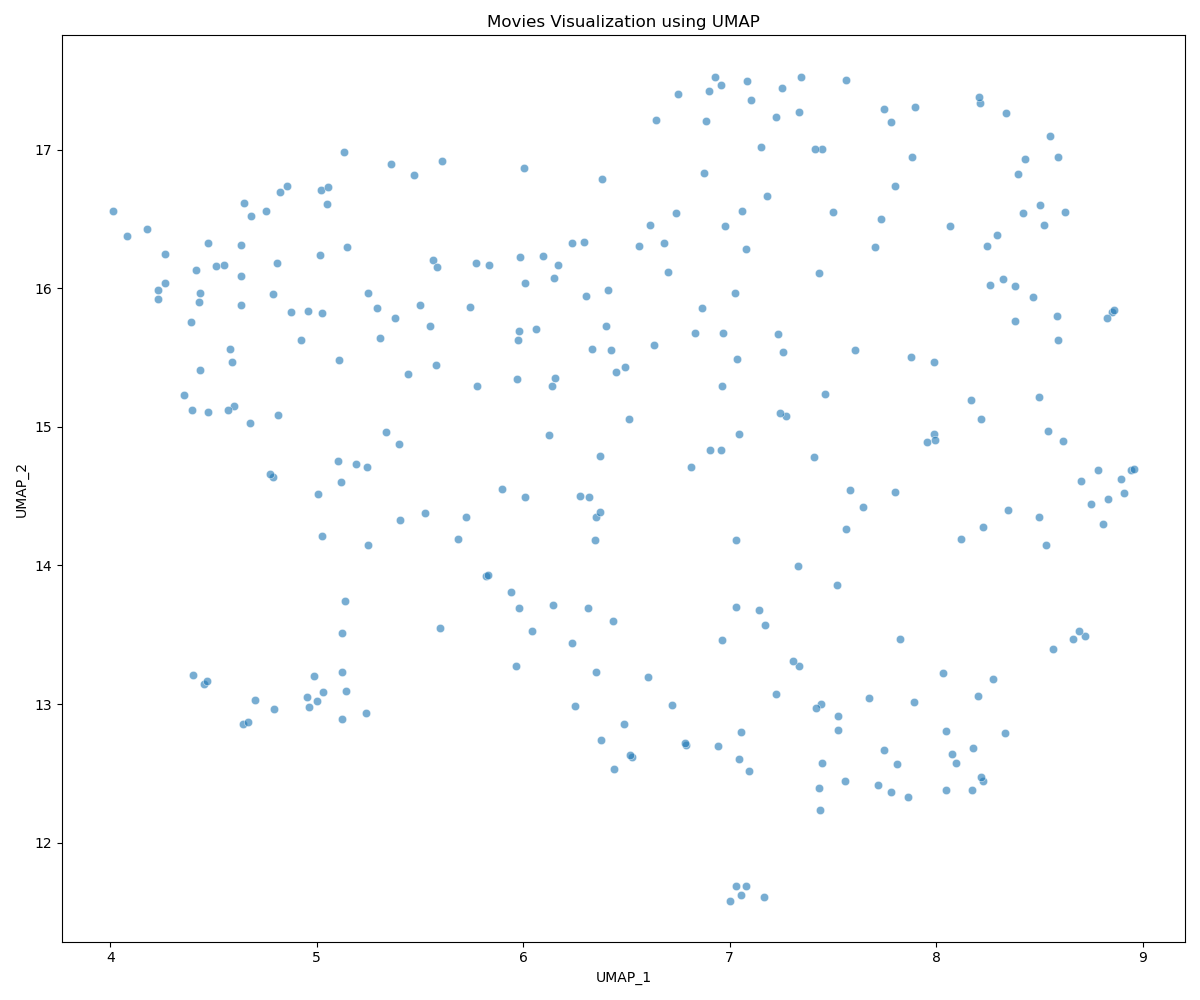
\includegraphics[width=0.8\linewidth]{umap_plot.png}
    \caption{UMAP Scatter Plot of Movie Embeddings}
  \end{figure}
\end{frame}

% Section: Results and Insights
\section{Results and Insights}
\subsection{Dataset Statistics}
\begin{frame}{Dataset Statistics}
  \begin{itemize}
    \item \textbf{Total Movies:} 1,500
    \item \textbf{Genres:} Western, Action, Fantasy
    \item \textbf{Average Runtime:} 106 minutes
    \item \textbf{Language Distribution:} Primarily English with select multilingual entries.
    \item \textbf{Library Availability:} 60\% of movies available in at least one library
  \end{itemize}
\end{frame}

\subsection{Embedding Insights}
\begin{frame}{Clustering Insights}
  \begin{itemize}
    \item \textbf{Genre Clusters:} Clear separation between Western, Action, and Fantasy movies in the embedding space.
    \item \textbf{Trend Analysis:}
      \begin{itemize}
        \item Release year trends showing the evolution of genres over time.
        \item Correlation between IMDb ratings and embedding distances, indicating viewer preferences.
      \end{itemize}
    \item \textbf{Library Availability Patterns:}
      \begin{itemize}
        \item Popular and highly-rated movies are more likely to be available in libraries.
        \item Niche genres have lower availability rates, highlighting areas for library collection expansion.
      \end{itemize}
  \end{itemize}
\end{frame}

\end{document}
